\chapter{Output Data Analysis}

\section{Introduction}

Nelle \textbf{simulation studies}, una parte significativa delle risorse disponibili viene spesso dedicata alla fase di modellazione del sistema e alla sua implementazione software. Tuttavia, in molti casi, un’attenzione relativamente modesta viene riservata alla corretta \textbf{analisi dei dati di output} prodotti dalla simulazione. Questo squilibrio può compromettere seriamente la validità e l’affidabilità dei risultati ottenuti.

Una pratica purtroppo comune consiste nell’eseguire una singola replica della simulazione e nel trattare le stime risultanti come se rappresentassero le vere caratteristiche del sistema modellato. In realtà, tali stime non sono valori deterministici, ma \textbf{realizzazioni di variabili casuali}, spesso caratterizzate da una varianza non trascurabile. Di conseguenza, una singola esecuzione della simulazione può produrre risultati significativamente diversi dai valori medi di lungo periodo del modello.

Questo aspetto introduce un rischio concreto di \textbf{inferenze errate}. In particolare, decisioni progettuali o operative basate su una singola osservazione simulativa possono risultare subottimali o addirittura fuorvianti. In termini probabilistici, esiste una non trascurabile probabilità che una specifica realizzazione della simulazione si discosti in modo rilevante dalle reali prestazioni attese del sistema.

Affinché i risultati di uno studio di simulazione abbiano un reale significato, è quindi essenziale adottare \textbf{tecniche statistiche appropriate} per la progettazione degli esperimenti e per l’analisi dei dati di output. Tali tecniche devono tenere conto delle peculiarità dei processi simulati, che spesso presentano caratteristiche di \textbf{non stazionarietà} e \textbf{autocorrelazione}.

A differenza delle osservazioni classiche utilizzate in molti contesti statistici, i dati di output di una simulazione non possono in generale essere considerati indipendenti e identicamente distribuiti (IID). Di conseguenza, le tecniche statistiche tradizionali basate su questa ipotesi non sono direttamente applicabili. L’output data analysis si pone quindi l’obiettivo di sviluppare e utilizzare metodi statistici in grado di fornire stime affidabili delle prestazioni del sistema e di quantificare l’incertezza associata a tali stime.

\section{Stochastic Processes}
\begin{wrapfigure}{r}{0.4\textwidth}
    \centering
    \vspace{-10pt}
    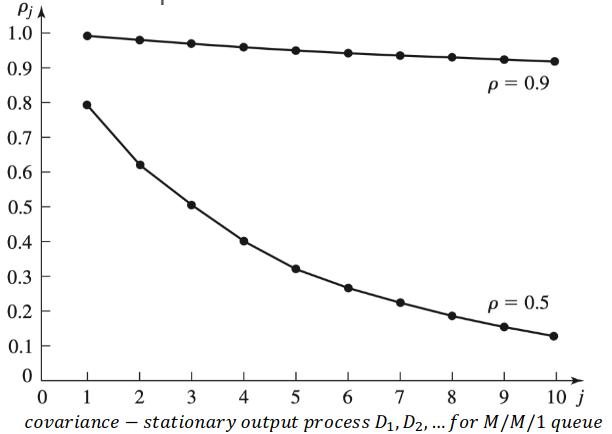
\includegraphics[width=\linewidth]{images/OD1.png}
    \label{fig:TDlambda}
    \vspace{-10pt}
\end{wrapfigure}
La maggior parte dei modelli di simulazione utilizza \textbf{variabili casuali} come input, ad esempio per descrivere i tempi di interarrivo, i tempi di servizio o le decisioni operative dei clienti. Di conseguenza, anche le \textbf{variabili di output} generate dalla simulazione sono di natura casuale. L’output di una simulazione non è quindi costituito da singole osservazioni indipendenti, ma da sequenze strutturate di variabili casuali.

In questo contesto, l’output della simulazione viene naturalmente descritto tramite un \textbf{processo stocastico}. Un processo stocastico è una collezione di variabili casuali ``simili’’ tra loro, ordinate nel tempo e definite su un medesimo spazio campionario. Formalmente, esso rappresenta l’evoluzione nel tempo di una certa grandezza casuale associata al sistema simulato.

Il \textbf{state space} di un processo stocastico è l’insieme di tutti i valori che le variabili casuali del processo possono assumere. A seconda della natura del tempo, i processi stocastici possono essere classificati come:
\begin{compactitemize}
    \item \textbf{discrete-time stochastic processes}, se l’indice temporale assume valori discreti;
    \item \textbf{continuous-time stochastic processes}, se l’evoluzione avviene su un asse temporale continuo.
\end{compactitemize}

Un esempio classico di processo stocastico generato da una simulazione è fornito da una coda \textbf{$M/M/1$}. In questo modello:
\begin{compactitemize}
    \item $A_1, A_2, \dots$ sono i tempi di interarrivo, variabili casuali IID;
    \item $S_1, S_2, \dots$ sono i tempi di servizio, anch’essi variabili casuali IID;
    \item la disciplina di servizio è FIFO.
\end{compactitemize}

Indicando con $D_1, D_2, \dots$ i ritardi (delay) sperimentati dai clienti, si ottiene un \textbf{processo stocastico a tempo discreto} che descrive l’evoluzione dei tempi di attesa nel sistema. Tali ritardi soddisfano la relazione ricorsiva:
\[
D_0 = 0, \qquad
D_{i+1} = \max\{D_i + S_i - A_{i+1},\, 0\}
\]
La simulazione realizza quindi una mappatura dalle variabili casuali di input $(A_i, S_i)$ al processo stocastico di output $(D_i)$.

Per poter trarre inferenze significative sul comportamento di un sistema a partire dai dati di output simulati, è spesso necessario introdurre alcune \textbf{ipotesi semplificative} sulla struttura del processo stocastico, anche quando tali ipotesi non sono perfettamente verificate nella pratica. Una delle ipotesi più utilizzate nell’output data analysis è quella di \textbf{covariance-stationarity}.

Un processo stocastico a tempo discreto $X_1, X_2, \dots$ si dice \textbf{covariance-stationary} se soddisfa le seguenti condizioni:
\begin{itemize}
    \item il valore atteso è costante nel tempo:
    \[
    \mu_i = \mu \quad \text{per } i = 1,2,\dots, \qquad -\infty < \mu < \infty;
    \]
    \item la varianza è costante e finita:
    \[
    \sigma_i^2 = \sigma^2 \quad \text{per } i = 1,2,\dots, \qquad \sigma^2 < \infty;
    \]
    \item la covarianza tra $X_i$ e $X_{i+j}$ dipende solo dal ritardo $j$ e non dall’istante $i$:
    \[
    C_{i,i+j} = \operatorname{Cov}(X_i, X_{i+j}) = C_j \quad \text{per } j = 1,2,\dots
    \]
\end{itemize}

In un processo covariance-stationary, quindi, la media e la varianza sono stazionarie nel tempo, mentre la dipendenza tra due osservazioni è funzione esclusivamente della loro separazione temporale, detta \textbf{lag}.

Per tali processi, la covarianza e la correlazione tra $X_i$ e $X_{i+j}$ vengono comunemente indicate rispettivamente con $C_j$ e $\rho_j$, dove:
\[
\rho_j = \frac{C_{i,i+j}}{\sigma_i \sigma_{i+j}} = \frac{C_j}{\sigma^2}
\]

Questa struttura rende i processi covariance-stationary particolarmente adatti all’analisi statistica dell’output di simulazione, poiché consente di caratterizzare la dipendenza temporale dei dati attraverso funzioni di autocovarianza e autocorrelazione, che giocano un ruolo centrale nelle tecniche di output data analysis.

\section{Transient and Steady-State Behaviour}

Si consideri un generico \textbf{processo stocastico di output} generato da una simulazione, indicato con $Y_1, Y_2, \dots$, dove $Y_i$ rappresenta l’osservazione dell’output al tempo (o indice) $i$. Il comportamento statistico di tale processo dipende in modo cruciale dalle \textbf{condizioni iniziali} del sistema.

Sia $I$ l’insieme delle condizioni iniziali della simulazione. Per ogni istante $i$, si definisce la funzione di distribuzione:
\[
F_i(y \mid I) = P(Y_i \le y \mid I)
\]
\begin{wrapfigure}{r}{0.4\textwidth}
    \centering
    \vspace{-10pt}
    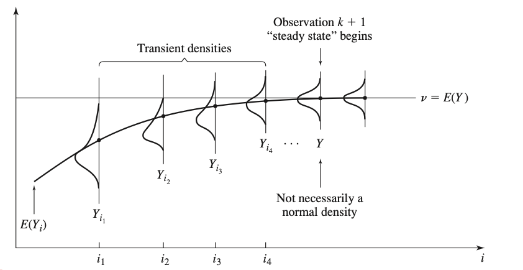
\includegraphics[width=\linewidth]{images/OD2.png}
    \label{fig:TDlambda}
    \vspace{-10pt}
\end{wrapfigure}
Tale funzione è detta \textbf{distribuzione transitoria} (transient distribution) del processo di output al tempo $i$, dato l’insieme di condizioni iniziali $I$.

In generale, durante la fase iniziale della simulazione, la distribuzione di $Y_i$ dipende fortemente dalle condizioni iniziali. Questa fase è detta \textbf{transient}. Tuttavia, per molte classi di sistemi stocastici stabili, l’influenza delle condizioni iniziali tende a diminuire nel tempo. Se vale che:
\[
F_i(y \mid I) \longrightarrow F(y) \quad \text{per } i \to \infty
\]
allora la distribuzione limite $F(y)$ è detta \textbf{steady-state distribution} del processo di output.

Una volta raggiunto lo steady-state, la distribuzione delle osservazioni non dipende più dalle condizioni iniziali. Inoltre, la sequenza di output $Y_{k+1}, Y_{k+2}, \dots$ non è in generale costituita da osservazioni indipendenti, ma forma un \textbf{processo covariance-stationary}. In particolare, la media e la varianza rimangono costanti nel tempo e la dipendenza tra osservazioni è funzione esclusivamente del lag.

Un aspetto fondamentale nell’output data analysis è la \textbf{velocità di convergenza} dallo stato transitorio allo steady-state. Tale velocità è fortemente influenzata dalle condizioni iniziali della simulazione. Condizioni iniziali ``lontane’’ dall’equilibrio possono produrre lunghi periodi transitori, introducendo bias significativi nelle stime delle misure di performance.
\begin{wrapfigure}{r}{0.4\textwidth}
    \centering
    \vspace{-10pt}
    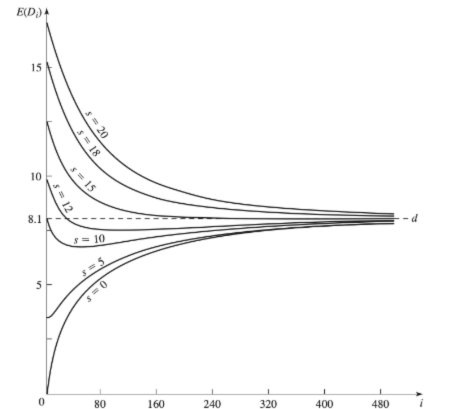
\includegraphics[width=\linewidth]{images/OD3.png}
    \label{fig:TDlambda}
    \vspace{-10pt}
\end{wrapfigure}
Per illustrare questo fenomeno, si consideri il processo stocastico dei ritardi $D_1, D_2, \dots$ in una coda \textbf{$M/M/1$} con server utilization pari a $\rho = 0.9$. Poiché il sistema è altamente carico, il tempo necessario per raggiungere lo steady-state può essere molto lungo. In particolare, se la simulazione viene avviata da uno stato vuoto ($D_0 = 0$), i ritardi iniziali risultano artificialmente bassi rispetto ai valori tipici di regime.

In tali condizioni, l’utilizzo diretto delle osservazioni iniziali per stimare le prestazioni del sistema porta a una sottostima sistematica dei ritardi medi. Questo esempio mette in evidenza l’importanza di distinguere correttamente tra fase transitoria e fase stazionaria e di adottare tecniche appropriate, come l’eliminazione del periodo di warm-up, per ridurre l’effetto delle condizioni iniziali sull’analisi dei dati di output.

\section{Types of Simulations and Output Analysis}

Le simulazioni possono essere classificate in due categorie fondamentali, a seconda della natura temporale del sistema studiato e degli obiettivi dell’analisi: \textbf{terminating simulations} e \textbf{nonterminating simulations}. Questa distinzione ha un impatto diretto sulle tecniche di output data analysis da utilizzare.

Una \textbf{terminating simulation} è caratterizzata dalla presenza di un evento naturale $E$ che determina la fine di ogni esecuzione, o \emph{replication}, della simulazione. Tale evento si verifica tipicamente quando il sistema viene completamente svuotato oppure quando viene raggiunto un orizzonte temporale prefissato, spesso imposto da vincoli organizzativi o gestionali.

In questo contesto, tutte le repliche della simulazione iniziano da condizioni iniziali comparabili e terminano al verificarsi dell’evento $E$. Di conseguenza, le variabili casuali di output ottenute dalle diverse repliche risultano \textbf{indipendenti e identicamente distribuite (IID)}, consentendo l’applicazione diretta delle tecniche statistiche classiche.

Un esempio tipico di terminating simulation è rappresentato da una \textbf{banca che chiude ogni sera}. Se la banca è aperta dalle 9:00 alle 17:00, l’obiettivo della simulazione può essere la stima della qualità del servizio offerto durante la giornata lavorativa. In questo caso, l’evento di terminazione può essere definito come:
\[
E = \{\text{sono trascorse almeno 8 ore di tempo simulato e il sistema è vuoto}\}
\]
Le condizioni iniziali della simulazione sono date dal numero di clienti presenti nel sistema all’istante $t = 0$.

Al contrario, una \textbf{nonterminating simulation} è una simulazione per la quale non esiste un evento naturale che ne determini la conclusione. Questo tipo di simulazione è tipicamente utilizzato quando l’obiettivo dello studio riguarda il \textbf{comportamento di lungo periodo} del sistema. In tali casi, l’attenzione è rivolta a misure di performance che sono caratteristiche della distribuzione stazionaria di un processo stocastico di output $Y_1, Y_2, \dots$.

Una misura di performance è detta \textbf{steady-state parameter} se è una caratteristica della steady-state distribution del processo di output. Un esempio classico è il valore atteso $E[Y]$ in regime stazionario.

Un esempio di nonterminating simulation è fornito da un \textbf{sistema manifatturiero} che opera su due turni giornalieri, per un totale di 16 ore al giorno, con work-in-process che viene trasferito da un giorno al successivo. In questo caso, l’operazione produttiva è essenzialmente continua e le condizioni finali di una giornata coincidono con le condizioni iniziali della successiva. Pertanto, non è possibile identificare un evento naturale di terminazione.

È importante osservare che molti sistemi reali non ammettono una vera steady-state distribution, poiché le loro caratteristiche possono variare nel tempo. Ad esempio, in un sistema di produzione, le regole di schedulazione o la configurazione dell’impianto possono essere modificate. Tuttavia, un \textbf{modello di simulazione}, che rappresenta un’astrazione della realtà, può essere costruito assumendo parametri invarianti nel tempo, rendendo possibile l’esistenza di una steady-state distribution.

Inoltre, uno stesso sistema può essere modellato come terminating o nonterminating a seconda degli obiettivi specifici dello studio di simulazione.

Infine, si consideri una nonterminating simulation associata a un processo stocastico di output $Y_1, Y_2, \dots$ che non possiede una steady-state distribution. In tali casi, una tecnica comune consiste nel suddividere l’asse temporale in intervalli contigui di uguale durata, detti \textbf{cycles}. Sia $Y_i^C$ la variabile casuale definita sul $i$-esimo ciclo, e si assuma che le variabili $Y_1^C, Y_2^C, \dots$ siano confrontabili.

Se il processo ciclico $Y_1^C, Y_2^C, \dots$ ammette una steady-state distribution $F_C$ e se $Y^C \sim F_C$, allora una misura di performance è detta \textbf{steady-state cycle parameter} se rappresenta una caratteristica della distribuzione $F_C$, come ad esempio il valore atteso:
\[
E[Y^C]
\]

Questo approccio consente di estendere l’analisi di steady-state anche a sistemi che, nel tempo continuo, non presentano una distribuzione stazionaria ben definita.

\section{Output Analysis for Terminating Simulations}

Si consideri una \textbf{terminating simulation}, ovvero una simulazione caratterizzata da un evento naturale di terminazione $E$ che definisce la durata di ciascuna esecuzione. Supponiamo di effettuare $n$ \textbf{repliche indipendenti} della simulazione, tutte con le stesse condizioni iniziali e lo stesso evento terminale.  
L’indipendenza tra le repliche è garantita utilizzando differenti stream di numeri casuali per ciascuna esecuzione.

Per semplicità, si assuma che vi sia una sola misura di performance di interesse. Sia $X_j$ la variabile casuale definita sulla $j$-esima replica, con $j = 1,2,\dots,n$. Poiché le repliche sono comparabili e indipendenti, le variabili $X_1, X_2, \dots, X_n$ possono essere considerate \textbf{IID}.

Un esempio tipico è il caso in cui $X_j$ rappresenti il \textbf{ritardo medio giornaliero} osservato nella $j$-esima replica di una simulazione bancaria:
\[
X_j = D_j = \frac{1}{N} \sum_{i=1}^{N} D_i
\]
dove $D_i$ è il ritardo del cliente $i$ durante quella giornata simulata.

L’obiettivo è stimare il vero valore medio:
\[
\mu = E[X]
\]
e costruire un \textbf{intervallo di confidenza} per $\mu$.

\section{Fixed-sample-size procedure}
Dato un numero fissato di repliche $n$, si utilizza la media campionaria:
\[
\bar{X}_n = \frac{1}{n} \sum_{j=1}^{n} X_j
\]
e la varianza campionaria:
\[
S^2(n) = \frac{1}{n-1} \sum_{j=1}^{n} (X_j - \bar{X}_n)^2
\]

Un intervallo di confidenza approssimato al livello $100(1-\alpha)\%$ per $\mu$ è dato da:
\[
\bar{X}_n \pm t_{n-1,\,1-\alpha/2} \sqrt{\frac{S^2(n)}{n}}
\]
dove $t_{n-1,\,1-\alpha/2}$ è il quantile della distribuzione $t$ di Student con $n-1$ gradi di libertà.

Uno svantaggio principale della procedura a numerosità fissata è che l’analista \textbf{non ha controllo diretto sulla precisione} dell’intervallo di confidenza. In particolare, la semilarghezza dell’intervallo dipende dalla varianza di $X$ e, per un dato $n$, può risultare eccessivamente grande.

\section{Precisione assoluta}
Si definisca $\beta$ come \textbf{errore assoluto} dell’estimatore:
\[
\beta = |\bar{X} - \mu|
\]
Se si effettuano repliche fino a quando la semilarghezza dell’intervallo di confidenza è minore o uguale a $\beta$, allora:
\[
P(|\bar{X} - \mu| \le \beta) \approx 1 - \alpha
\]
ossia l’estimatore $\bar{X}$ ha errore assoluto al più pari a $\beta$ con probabilità approssimativamente $1-\alpha$.

Il numero di repliche richiesto può essere stimato come:
\[
n_\beta^* = \min \left\{ i \ge n :
t_{i-1,\,1-\alpha/2} \sqrt{\frac{S^2(n)}{i}} \le \beta \right\}
\]
In pratica, tale valore viene determinato in modo iterativo, aggiornando progressivamente la stima della varianza.

\section{Sequential procedure e precisione relativa}
Un approccio alternativo è la \textbf{procedura sequenziale}, in cui le repliche vengono aggiunte una alla volta. Si definisce così l’errore relativo:
\[
\gamma = \frac{|\bar{X} - \mu|}{\mu}
\]

La procedura è la seguente:
\begin{enumerate}
    \item eseguire un numero iniziale di repliche $n_0 \ge 10$;
    \item calcolare $\bar{X}(n)$ e la semilarghezza dell’intervallo:
    \[
    \delta_{n,\alpha} =
    t_{n-1,\,1-\alpha/2} \sqrt{\frac{S^2(n)}{n}};
    \]
    \item se $\delta_{n,\alpha} / \bar{X}(n) \le \gamma$, allora $\bar{X}(n)$ è accettato come stima di $\mu$;
    \item altrimenti, incrementare $n$ di una unità, eseguire una nuova replica e tornare al passo precedente.
\end{enumerate}

È importante notare che in questa procedura la stima della varianza viene aggiornata dopo ogni replica e che il numero totale di repliche richieste è esso stesso una \textbf{variabile casuale}. Questo approccio consente un controllo diretto della precisione della stima, rendendolo particolarmente adatto all’analisi dell’output di simulazioni terminating.

\section{Estimating Other Measures of Performance}
\begin{wrapfigure}{r}{0.4\textwidth}
    \centering
    \vspace{-10pt}
    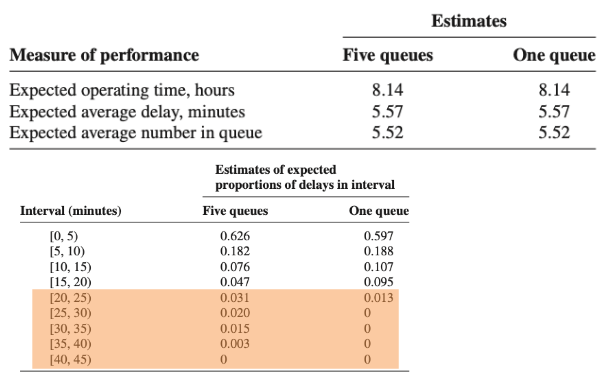
\includegraphics[width=\linewidth]{images/OD4.png}
    \label{fig:TDlambda}
    \vspace{-10pt}
\end{wrapfigure}
Valutare sistemi o politiche alternative esclusivamente sulla base del \textbf{valore medio} di una misura di performance può talvolta condurre a conclusioni fuorvianti. In molte applicazioni di operations e supply chain management, è infatti rilevante considerare anche \textbf{misure non medie}, come probabilità, proporzioni o percentuali di tempo in cui il sistema soddisfa determinati requisiti di prestazione.

Le \textbf{proporzioni} rappresentano una classe importante di misure di performance. Sia $X$ una variabile casuale definita su una singola replica di una simulazione terminating. Si supponga di voler stimare la probabilità:
\[
p = P(X \in B),
\]
dove $B \subset \mathbb{R}$ è un insieme di valori di interesse. Ad esempio, $B$ potrebbe rappresentare l’insieme dei valori per cui il ritardo supera una certa soglia, oppure i valori per cui il livello di servizio è ritenuto accettabile.

Si effettuino $n$ repliche indipendenti della simulazione e si indichino con $X_1, X_2, \dots, X_n$ le corrispondenti osservazioni, che possono essere considerate \textbf{IID}. Sia:
\[
S = \sum_{j=1}^{n} \mathbb{I}\{X_j \in B\}
\]
il numero di osservazioni che cadono nell’insieme $B$, dove $\mathbb{I}\{\cdot\}$ è la funzione indicatrice.

Poiché ciascuna osservazione ha probabilità $p$ di appartenere a $B$, la variabile casuale $S$ segue una \textbf{distribuzione binomiale} con parametri $n$ e $p$. Un estimatore non distorto di $p$ è quindi dato dalla proporzione campionaria:
\[
\hat{p} = \frac{S}{n}
\]

Per $n$ sufficientemente grande, la distribuzione di $\hat{p}$ può essere approssimata da una distribuzione normale. Un intervallo di confidenza approssimato al livello $100(1-\alpha)\%$ per la probabilità $p$ è allora:
\[
\hat{p} \pm z_{1-\alpha/2} \sqrt{\frac{\hat{p}(1-\hat{p})}{n}}
\]
dove $z_{1-\alpha/2}$ è il quantile della distribuzione normale standard.

Questo approccio consente di stimare in modo rigoroso probabilità e proporzioni di interesse, fornendo una visione più completa delle prestazioni del sistema rispetto alla sola analisi dei valori medi. In particolare, esso è particolarmente utile nel confronto tra sistemi alternativi, quando la probabilità di eventi critici o di violazioni di soglie operative riveste un ruolo centrale nel processo decisionale.

\section{Statistical Analysis for Steady-State Parameters}
\begin{wrapfigure}{r}{0.4\textwidth}
    \centering
    \vspace{-10pt}
    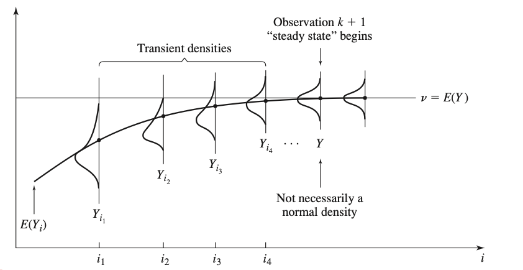
\includegraphics[width=\linewidth]{images/OD2.png}
    \label{fig:TDlambda}
    \vspace{-10pt}
\end{wrapfigure}
Si consideri un \textbf{processo stocastico di output} $Y_1, Y_2, \dots$ ottenuto da una singola esecuzione di una \textbf{nonterminating simulation}. Supponiamo che la distribuzione delle osservazioni converga nel tempo, ossia che:
\[
P(Y_i \le y) = F_i(y) \longrightarrow F(y) = P(Y \le y)
\quad \text{per } i \to \infty,
\]
dove $Y$ è la variabile casuale di interesse in \textbf{steady-state}, con funzione di distribuzione $F$.

Una quantità $\phi$ è detta \textbf{steady-state parameter} se rappresenta una caratteristica della distribuzione stazionaria di $Y$. Esempi tipici di steady-state parameters includono:
\begin{compactitemize}
    \item il valore atteso $E[Y]$;
    \item una probabilità del tipo $P(Y \le y)$;
    \item un quantile della distribuzione di $Y$.
\end{compactitemize}

Una difficoltà fondamentale nella stima di $\phi$ è dovuta al fatto che, in generale, la distribuzione delle osservazioni iniziali $Y_i$ non coincide con la distribuzione stazionaria $F$. Questo accade perché non è normalmente possibile scegliere condizioni iniziali $I$ che siano realmente rappresentative del comportamento di steady-state del sistema.

La conseguenza diretta è che uno stimatore di $\phi$ basato sulle osservazioni $Y_1, Y_2, \dots, Y_m$ risulta \textbf{non rappresentativo} del regime stazionario. Ad esempio, la media campionaria:
\[
\bar{Y}_m = \frac{1}{m} \sum_{i=1}^{m} Y_i
\]
è un estimatore \textbf{biased} del valore atteso stazionario $E[Y]$ per qualunque valore finito di $m$. Questo fenomeno è noto come \textbf{problem of the initial transient}, o anche \textbf{startup problem}.

Per chiarire questo aspetto, si consideri il processo dei ritardi $D_1, D_2, \dots$ in una coda \textbf{$M/M/1$} con server utilization $\rho < 1$. Dalla teoria delle code è noto che la distribuzione stazionaria del ritardo $D$ è:
\[
P(D \le y) = 1 - \rho + \rho\left(1 - e^{-(\mu - \lambda)y}\right).
\]

Se il numero di clienti presenti nel sistema all’istante iniziale $t=0$ è pari a zero, allora $D_1 = 0$ e, più in generale, vale che:
\[
E[D_i] \neq E[D] = d \quad \text{per ogni } i,
\]
ossia nessuna delle osservazioni iniziali ha media uguale al valore medio stazionario.

Al contrario, se il numero iniziale di clienti nel sistema è scelto in accordo con la \textbf{distribuzione stazionaria del numero di clienti nel sistema}, allora le osservazioni risultano immediatamente rappresentative del regime di steady-state, e vale che:
\[
P(D_i \le y) = P(D \le y), \qquad E[D_i] = d.
\]

Questo esempio evidenzia come la scelta delle condizioni iniziali influenzi in modo sostanziale l’analisi statistica dei parametri stazionari e motiva la necessità di tecniche specifiche per gestire il problema del transitorio iniziale nelle simulazioni nonterminating.

\section{The Problem of the Initial Transient}
\begin{wrapfigure}{r}{0.4\textwidth}
    \centering
    \vspace{-10pt}
    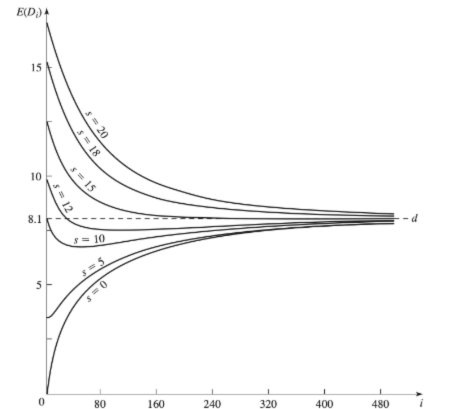
\includegraphics[width=\linewidth]{images/OD3.png}
    \label{fig:TDlambda}
    \vspace{-10pt}
\end{wrapfigure}
Si supponga di voler stimare il \textbf{valore medio in steady-state}:
\[
\nu = E[Y],
\]
che può essere formalmente definito come:
\[
\nu = \lim_{i \to \infty} E[Y_i],
\]
dove $Y_1, Y_2, \dots$ è un processo stocastico di output generato da una nonterminating simulation.

La conseguenza più rilevante del \textbf{problema del transitorio iniziale} è che, in generale,
\[
E[\bar{Y}_m] \neq \nu,
\]
dove:
\[
\bar{Y}_m = \frac{1}{m} \sum_{i=1}^{m} Y_i
\]
è la media campionaria calcolata sulle prime $m$ osservazioni. Ciò implica che, per qualunque valore finito di $m$, la media campionaria risulta un estimatore \textbf{biased} del valore medio stazionario.

La tecnica più comunemente adottata per ridurre l’effetto del transitorio iniziale è il cosiddetto \textbf{warming up} del modello, noto anche come \textbf{initial-data deletion}. L’idea è quella di eliminare un certo numero di osservazioni iniziali, che sono maggiormente influenzate dalle condizioni iniziali del sistema, e utilizzare solo le osservazioni rimanenti per stimare $\nu$.

Formalmente, fissato un intero $l \ge 0$, si definisce lo stimatore:
\[
\bar{Y}_{m,l} = \frac{1}{m-l} \sum_{i=l+1}^{m} Y_i.
\]

L’intuizione alla base di questo approccio è che $\bar{Y}_{m,l}$ dovrebbe presentare un bias inferiore rispetto a $\bar{Y}_m$, poiché le osservazioni all’inizio della simulazione potrebbero non essere rappresentative del comportamento in steady-state.

La scelta del \textbf{warm-up period} $l$ rappresenta tuttavia un problema delicato. In particolare, si desidera selezionare $l$ (e $m$) in modo tale che:
\[
E[\bar{Y}_{m,l}] \approx \nu.
\]

Se $l$ e $m$ sono scelti troppo piccoli, il bias residuo dovuto al transitorio iniziale può essere ancora significativo, compromettendo l’accuratezza della stima. Al contrario, se $l$ è scelto troppo grande, si eliminano inutilmente molte osservazioni, con il risultato di aumentare la varianza di $\bar{Y}_{m,l}$.

È quindi necessario trovare un compromesso tra riduzione del bias e contenimento della varianza. Una tecnica semplice e di uso generale per determinare un valore appropriato di $l$ è rappresentata da una \textbf{procedura grafica}, che consente di individuare empiricamente il punto a partire dal quale il processo di output può essere considerato sufficientemente vicino al regime stazionario.

\section{Welch’s Procedure}
\begin{wrapfigure}{r}{0.4\textwidth}
    \centering
    \vspace{-10pt}
    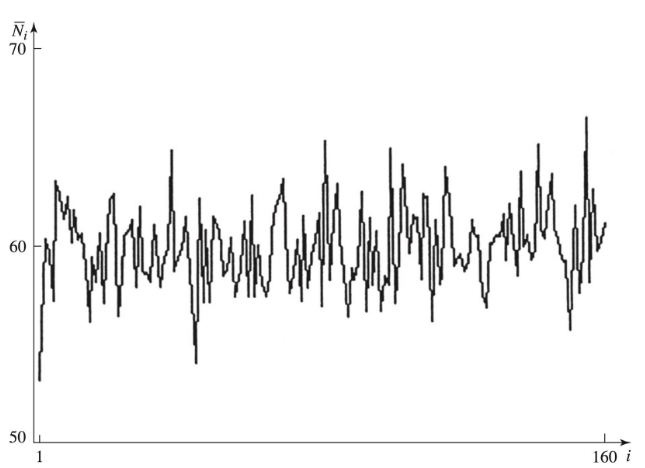
\includegraphics[width=\linewidth]{images/OD5.png}
    \label{fig:TDlambda}
    \vspace{-10pt}
\end{wrapfigure}
Come discusso in precedenza, una tecnica semplice e di uso generale per determinare il
\textbf{warm-up period} $l$ è una procedura grafica, nota come \textbf{Welch’s procedure}.
Lo stimatore utilizzato per il valore medio in steady-state è:
\[
\bar{Y}_{m,l} = \frac{1}{m-l} \sum_{i=l+1}^{m} Y_i,
\]
dove $l$ rappresenta il numero di osservazioni iniziali eliminate e $m$ la lunghezza totale
della simulazione.

L’obiettivo della Welch’s procedure è determinare un valore di $l$ tale che:
\[
E[\bar{Y}_{m,l}] \approx \nu,
\]
dove $\nu$ è il valore medio in steady-state. In modo equivalente, il problema consiste
nell’individuare l’istante a partire dal quale la curva del valore atteso transitorio
$E[Y_i]$ si stabilizza (``flattens-out'') attorno al livello $\nu$.

Poiché è in generale molto difficile identificare tale punto a partire da una singola
replica, a causa dell’elevata variabilità del processo stocastico, la Welch’s procedure
utilizza più repliche e tecniche di smoothing.

La procedura può essere descritta come segue:
\begin{enumerate}
    \item eseguire $n$ repliche indipendenti della simulazione ($n \ge 5$), ciascuna di
    lunghezza $m$ sufficientemente grande. Sia $Y_{ji}$ l’osservazione $i$-esima della
    $j$-esima replica;
    \item calcolare, per ogni $i$, la media sulle repliche:
    \[
    \tilde{Y}_i = \frac{1}{n} \sum_{j=1}^{n} Y_{ji},
    \]
    che soddisfa $E[\tilde{Y}_i] = E[Y_i]$ e
    $\operatorname{Var}(\tilde{Y}_i) = \operatorname{Var}(Y_i)/n$;
    \item per ridurre le oscillazioni ad alta frequenza, definire una media mobile
    $\tilde{Y}_i^{(w)}$:
    \[
    \tilde{Y}_i^{(w)} =
    \begin{cases}
    \displaystyle
    \frac{1}{2w+1} \sum_{s=-w}^{w} \tilde{Y}_{i+s}, 
    & i = w+1, \dots, m-w, \\[8pt]
    \displaystyle
    \frac{1}{2i+1} \sum_{s=-(i-1)}^{i-1} \tilde{Y}_{i+s},
    & i = 1, \dots, w;
    \end{cases}
    \]
    \item tracciare il grafico di $\tilde{Y}_i^{(w)}$ e scegliere $l$ come il primo indice
    temporale oltre il quale la curva appare stabilizzata.
\end{enumerate}

Il valore di $l$ così ottenuto viene quindi utilizzato nello stimatore
$\bar{Y}_{m,l}$ per eliminare l’effetto del transitorio iniziale nelle analisi di
steady-state.

\begin{figure}[H]
    \centering
    \begin{minipage}{0.5\textwidth}
        \centering
        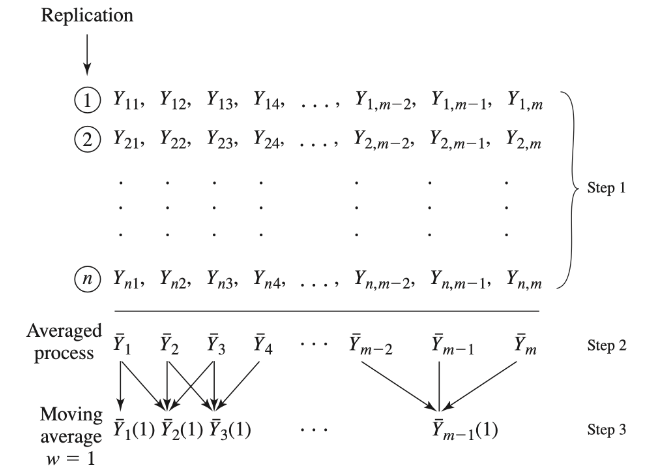
\includegraphics[width=\textwidth]{images/OD6.png}
        \label{fig:STMCR}
    \end{minipage}
    \hfill
    \begin{minipage}{0.45\textwidth}
        \centering
        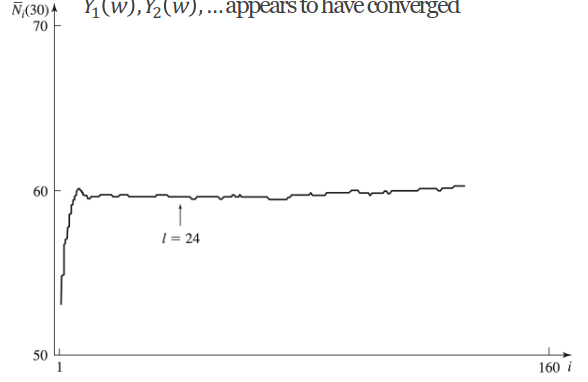
\includegraphics[width=\textwidth]{images/OD7.png}
        \label{fig:STMCR}
    \end{minipage}
    \label{STMCR}
\end{figure}

\section{Replication/Deletion Approach}

Una volta determinato il valore del \textbf{warm-up period} $l$ mediante la Welch’s graphical
procedure, è possibile utilizzare il \textbf{replication/deletion approach} per ottenere
una stima puntuale e un intervallo di confidenza per il valore medio in steady-state
\[
\nu = E[Y].
\]

L’idea di base consiste nell’eseguire più repliche indipendenti della simulazione e,
all’interno di ciascuna replica, eliminare le osservazioni iniziali corrispondenti al
periodo transitorio.

Si effettuino $n'$ repliche indipendenti della simulazione, ciascuna di lunghezza $m'$,
con $m' \gg l$. Si indichi con $Y_{ji}$ l’osservazione $i$-esima della $j$-esima replica.
Per ciascuna replica, si definisce la variabile casuale:
\[
X_j = \frac{1}{m' - l} \sum_{i=l+1}^{m'} Y_{ji},
\qquad j = 1,2,\dots,n'.
\]

Poiché le osservazioni iniziali sono state eliminate, ciascuna variabile $X_j$ può essere
considerata una stima del valore medio in steady-state, e vale approssimativamente:
\[
E[X_j] \approx \nu.
\]

Assumendo l’indipendenza tra le repliche, le variabili $X_1, X_2, \dots, X_{n'}$ possono
essere trattate come \textbf{IID}. Di conseguenza, è possibile applicare le tecniche
statistiche standard per stimare $\nu$.

La media campionaria:
\[
\bar{X}_{n'} = \frac{1}{n'} \sum_{j=1}^{n'} X_j
\]
fornisce una stima puntuale di $\nu$, mentre la varianza campionaria:
\[
S^2(n') = \frac{1}{n'-1} \sum_{j=1}^{n'} (X_j - \bar{X}_{n'})^2
\]
è utilizzata per quantificare la variabilità tra le repliche.

Un intervallo di confidenza approssimato al livello $100(1-\alpha)\%$ per il valore medio
in steady-state è quindi dato da:
\[
\bar{X}_{n'} \pm t_{n'-1,\,1-\alpha/2} \sqrt{\frac{S^2(n')}{n'}}.
\]

Il replication/deletion approach combina quindi due idee fondamentali dell’output data
analysis: l’eliminazione del transitorio iniziale all’interno di ciascuna replica e
l’utilizzo di repliche indipendenti per ottenere stime affidabili e intervalli di
confidenza statisticamente validi per i parametri di steady-state.

\section{Estimating Other Measures of Performance}

Come discusso in precedenza, il valore medio di una misura di performance non è
sempre sufficiente a descrivere in modo completo il comportamento di un sistema.
In molti contesti applicativi, basarsi esclusivamente sulla media può condurre a
conclusioni fuorvianti, specialmente quando la distribuzione delle prestazioni
presenta elevata variabilità o code pesanti.

Per questo motivo, risulta spesso necessario stimare \textbf{parametri di steady-state}
$\phi$ diversi dalla media
\[
\nu = E[Y],
\]
dove $Y$ rappresenta la variabile casuale di interesse in steady-state.

Un esempio particolarmente importante è la stima di una \textbf{probabilità di
steady-state}. Si supponga di voler stimare:
\[
p = P(Y \in B),
\]
dove $B$ è un sottoinsieme dei numeri reali che rappresenta una condizione di
interesse (ad esempio, un ritardo superiore a una certa soglia).

Tale problema può essere ricondotto alla stima di una media introducendo una
variabile indicatrice $Z$ definita come:
\[
Z =
\begin{cases}
1 & \text{se } Y \in B, \\
0 & \text{altrimenti}.
\end{cases}
\]

Per definizione, vale che:
\[
P(Y \in B) = P(Z = 1).
\]
Osservando che:
\[
E[Z] = 1 \cdot P(Z = 1) + 0 \cdot P(Z = 0) = P(Z = 1),
\]
si ottiene:
\[
P(Y \in B) = E[Z].
\]

Ne segue che la stima di una probabilità di steady-state è un caso particolare
della stima del valore medio di una variabile casuale. Di conseguenza, tutte le
tecniche sviluppate per la stima della media in steady-state, come il
replication/deletion approach o altre procedure di output data analysis, possono
essere applicate direttamente anche alla stima di probabilità e, più in generale,
di altri parametri di performance basati su funzioni indicatrici.

Questo approccio consente di estendere in modo naturale l’analisi delle prestazioni
a misure più informative rispetto alla sola media, migliorando la capacità di
valutare e confrontare sistemi o politiche alternative.

\section{Statistical Analysis for Steady-State Cycle Parameters}

In alcuni sistemi reali, il processo di output
\[
Y_1, Y_2, \dots
\]
non ammette una distribuzione di steady-state. Ciò può avvenire, ad esempio, quando
le caratteristiche del sistema evolvono nel tempo oppure quando il processo presenta
andamenti ciclici intrinseci.

Si supponga tuttavia che sia possibile individuare una \textbf{definizione appropriata
di ciclo} tale per cui, suddividendo l’evoluzione del sistema in cicli consecutivi,
il processo associato ai cicli:
\[
Y_1^{C}, Y_2^{C}, \dots
\]
ammetta una distribuzione di steady-state, indicata con $F_C$. In questo caso, la
variabile casuale $Y^{C}$, con distribuzione $F_C$, rappresenta l’output di interesse
a livello di ciclo.

Una \textbf{steady-state cycle parameter} è quindi definita come una qualsiasi
caratteristica della distribuzione di $Y^{C}$, ad esempio:
\[
E[Y^{C}], \quad P(Y^{C} \le y), \quad \text{oppure un quantile di } Y^{C}.
\]

È importante osservare che la stima di un parametro di steady-state a livello di ciclo
non introduce concetti statisticamente nuovi: essa rappresenta semplicemente un
\textbf{caso particolare della stima di un parametro di steady-state}. Di conseguenza,
tutte le tecniche sviluppate per l’analisi statistica dei parametri di steady-state
possono essere applicate direttamente alle variabili casuali di ciclo
\[
Y_1^{C}, Y_2^{C}, \dots
\]

In pratica, una volta definito correttamente il ciclo e verificata l’esistenza di una
distribuzione stazionaria per il processo ciclico, l’output data analysis procede in
modo del tutto analogo ai casi già studiati, consentendo di ottenere stime puntuali e
intervalli di confidenza per i parametri di interesse.

\begin{figure}[H]
    \centering
    \begin{minipage}{0.5\textwidth}
        \centering
        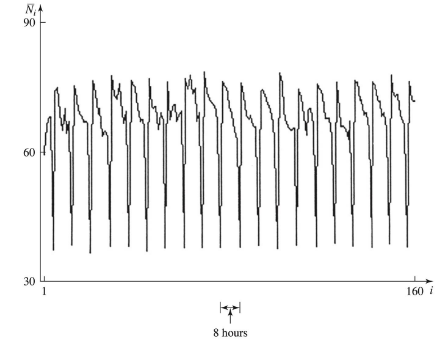
\includegraphics[width=\textwidth]{images/OD8.png}
        \label{fig:STMCR}
    \end{minipage}
    \hfill
    \begin{minipage}{0.45\textwidth}
        \centering
        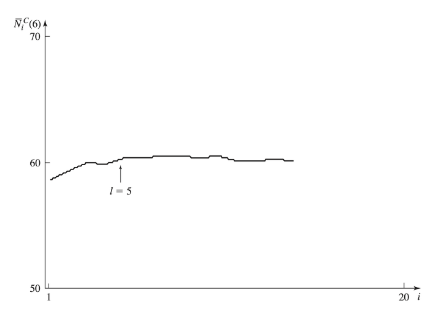
\includegraphics[width=\textwidth]{images/OD9.png}
        \label{fig:STMCR}
    \end{minipage}
    \label{STMCR}
\end{figure}

\section{Multiple Measures of Performance}

Fino a questo punto sono state considerate procedure statistiche per la costruzione
di intervalli di confidenza relativi a una singola misura di performance. Tuttavia,
nelle applicazioni reali della simulazione è frequente che l’analista sia interessato
a valutare \textbf{più misure di performance simultaneamente}, come ritardi medi,
utilization delle risorse, probabilità di congestione e throughput.

Si supponga che, per ciascuna misura di performance $\mu_s$, con
\[
s = 1,2,\dots,k,
\]
sia stato costruito un intervallo di confidenza $I_s$ al livello
$100(1-\alpha_s)\%$.

L’interesse è rivolto alla probabilità che \emph{tutti} gli intervalli di confidenza
contengano simultaneamente i rispettivi valori veri. Tale probabilità è limitata
inferiormente dalla \textbf{disuguaglianza di Bonferroni}, secondo la quale vale:
\[
P\left( \mu_s \in I_s \text{ per tutti } s = 1,2,\dots,k \right)
\;\ge\;
1 - \sum_{s=1}^{k} \alpha_s.
\]

Questa relazione mostra che, all’aumentare del numero di misure di performance $k$,
la probabilità complessiva che tutti gli intervalli siano simultaneamente corretti
può ridursi in modo significativo.

Ad esempio, se si costruiscono $k=10$ intervalli di confidenza al $90\%$ per ciascuna
misura, si ha $\alpha_s = 0.1$ per ogni $s$ e quindi:
\[
1 - \sum_{s=1}^{10} \alpha_s = 1 - 1 = 0.
\]
In questo caso, non è possibile garantire alcun livello di confidenza complessivo
positivo per l’insieme degli intervalli, nonostante ciascun intervallo singolo abbia
un’elevata affidabilità.

Una \textbf{soluzione pratica} consiste nello scegliere i livelli di significatività
$\alpha_s$ in modo tale che:
\[
\sum_{s=1}^{k} \alpha_s = \alpha,
\]
dove $\alpha$ rappresenta il livello di significatività complessivo desiderato.

Ad esempio, se si desidera un livello di confidenza globale di almeno $90\%$
($\alpha = 0.1$) per $k=10$ misure di performance, è possibile costruire dieci
intervalli di confidenza al $99\%$ per ciascuna misura. In questo modo, la probabilità
che tutti gli intervalli contengano i rispettivi valori veri è garantita essere almeno
pari al $90\%$.

Lo svantaggio di questo approccio è che i singoli intervalli di confidenza risultano
più ampi rispetto a quelli costruiti senza tener conto del problema della
simultaneità. Per questo motivo, una raccomandazione pratica è quella di limitare il
numero di misure di performance considerate simultaneamente, tipicamente a
\[
k \le 10.
\]

Questa analisi evidenzia l’importanza di considerare la dipendenza tra inferenze
statistiche quando si valutano più indicatori di performance all’interno di uno
studio di simulazione.
